\documentclass[12pt]{article}

\usepackage{url}
\usepackage{fullpage}
\usepackage{amssymb,amsfonts}
\usepackage{amsmath}
\newcommand{\eps}{\varepsilon}
\newcommand{\R}{\mathbb{R}}

\usepackage{listings}
\usepackage{color}
\usepackage{graphicx}

\usepackage{varwidth}

\usepackage{longtable}

\usepackage{hyperref}
\hypersetup{
    linktoc=all,     %set to all if you want both sections and subsections linked
    colorlinks=true,
    linkcolor=blue,
    filecolor=magenta,      
    urlcolor=cyan,
}

\definecolor{dkgreen}{rgb}{0,0.6,0}
\definecolor{gray}{rgb}{0.5,0.5,0.5}
\definecolor{mauve}{rgb}{0.58,0,0.82}

\lstset{frame=tb,
  language=Python,
  aboveskip=3mm,
  belowskip=3mm,
  showstringspaces=false,
  columns=flexible,
  basicstyle={\small\ttfamily},
  numbers=none,
  numberstyle=\tiny\color{gray},
  keywordstyle=\color{blue},
  commentstyle=\color{dkgreen},
  stringstyle=\color{mauve},
  breaklines=true,
  breakatwhitespace=true,
  tabsize=3
}

\usepackage[toc,page]{appendix}

\DeclareMathOperator*{\E}{\mathbb{E}}
\let\Pr\relax
\DeclareMathOperator*{\Pr}{\mathbb{P}}

\DeclareMathOperator*{\Lap}{\text{Lap}}

\DeclareMathOperator*{\Geo}{\text{Geo}}

\def\cl{\lstinline}

\title{CS 208 Homework 3}
\author{Andrew Shackelford}
\date{April 2, 2019}
\setcounter{tocdepth}{3}

\begin{document}

\maketitle

\textbf{All code and figures are available \href{https://github.com/andrew-shackelford/cs208/tree/master/3}{here}}.

{
  \hypersetup{linkcolor=black, hidelinks}
  \tableofcontents
}

\newpage

\section{Problem 1}

\subsection{Part A}

\noindent

By the definition of Lipschitz constants, a transformation $T$ is $c$-Lipschitz if and only if:

$$\forall x, x' d(T(x), T(x')) \leq c \cdot d(x, x')$$

Let us consider the transformation described in this mechanism, where we trim the dataset to the 5th and 95th percentiles. Any difference in the datasets $x$ and $x'$ can only change the transformed datasets $T(x)$ and $T(x')$ by the same amount. To prove this, we can simply look at how the mechanism works.

\medskip

The change of one row of a dataset can only change what rows are contained in the transformed dataset by one -- if the changed row was not in the trimmed dataset, it could now be included and push one row out, or vice versa. Since the number of rows in the dataset is the same, we know the size of the trimmed dataset is the same. As a result, the distance between the transformed datasets is 1, the same as the distance between the original datasets.

\medskip

Now we will look at adding or deleting a row. If we add a row, then the number of rows in the trimmed dataset either increases by 1 or stays the same. If the number of rows stays the same, this is analogous to changing one row of the dataset, and the distance between the transformed datasets is 1. If the number of rows increases by 1, then all of the original rows in the transformed dataset must remain, and we simply add one, thus giving us a distance of 1. If we delete a row and the number of rows stays the same, then the distance accordingly is still 1. Lastly, if the number of rows decreases by 1, we know that the transformed dataset still differs by 1, because a smaller transformed dataset could not include any new rows. As a result, the distance between the transformed datasets is 1, the same as the distance between the original datasets.

\medskip

We have shown that in all cases the distance between two transformed datasets with distance 1 is still 1, thus giving us a Lipschitz constant of 1. Since $M$ is the standard Laplace mechanism applied to a transformation with a Lipschitz constant of $c = 1$, $M$ is $(c \cdot \epsilon)$-DP, or just $\epsilon$-DP.

\medskip

To examine the code for this mechanism, see the \cl{part_a()} function of \cl{problem_1.py}, located at Appendix \ref{appendix:problem_1}.

\subsection{Part B}

\noindent

\textbf{Proof by contradiction.}

\bigskip

Consider a scenario where $D, n = 100$. Let $x$ contain 95 `1's and 5 `100's. In this case, the 95th percentile is equal to 1, so every datapoint is clipped to a maximum of 1, and thus the mean of $x = 1$. Now, consider us changing a datapoint from 1 to 100. This would change the 95th percentile to 100, and no datapoints would be clipped any longer. As a result, the mean would change by $\frac{99}{n} \cdot 5$ for the 5 `100s' that were not already clipped. As a result the mean will change by$\frac{5 \cdot 99}{100} = 4.95$.

\medskip

However, for a release with Laplace noise to be $\epsilon$-differentially private, the scale of the Laplace noise must be $\geq \frac{GS_q}{\epsilon}$. With our given mechanism, this means that $GS_q$ must be $\leq \frac{D}{n}$. However, our example above demonstrates a global sensitivity of 4.95, while $\frac{D}{n} = \frac{100}{100} = 1$. Since we demonstrated that this mechanism has a global sensitivity greater than what we account for with our Laplace noise, we have proven that this mechanism is not differentially private.

\subsection{Part C}

\noindent

For this part, I modified the exponential mechanism's utility function $u(x, y, t)$ to return $n - \alpha$, where $n = \text{len}(x)$, and $\alpha$ is the number of elements between $y$ and the $t$'th percentile of $x$. This way the utility function is strictly increasing as $y$ approaches the $t$'th percentile of $x$, and is defined for any $t \in [0, 100]$. When implementing the exponential mechanism, I chose to sort the elements of the dataset and assignment the same weight to all elements of each interval between $x_{i_j}$ and $x_{i_{j+1}}$. Also, since the utilities for each $(x, y, t)$ tuple do not change between runs, I used a dictionary to keep track of each $u(x, y, t)$ so that I don't have to recalculate the utilities on each trial. To examine the code for this function, see the \cl{part_c()} function of \cl{problem_1.py}, located at Appendix \ref{appendix:problem_1}.

\subsection{Part D}

\noindent

See the \cl{part_d()} function of \cl{problem_1.py}, located at Appendix \ref{appendix:problem_1}.

\subsection{Part E}

\noindent

Consider a traditional Laplace mechanism for the mean where we pass in clamping values $a$ and $b$ based on our priors. As proven many times before, this mechanism is $\epsilon$-DP, since $a$ and $b$ are independent of the data. This mechanism is functionally identical to the traditional Laplace mechanism except that $a$ and $b$ are differentially private estimates of the 5th and 95th percentiles. Since differential privacy is closed under post-processing, the use of $\hat{P}_{.05}$ and $\hat{P}_{.95}$ in any additional function cannot cause any additional privacy loss. Therefore, their use as clamping boundaries does not have any detrimental privacy benefits. As a result, through the composition of three $\frac{\epsilon}{3}$-DP functions, this mechanism is $\epsilon$-DP.

\subsection{Part F}

\subsubsection{Process}

See the \cl{part_f_experiment()}, \cl{part_f_analysis()}, and \cl{part_f_graph()} functions of \cl{problem_1.py}, located at Appendix \ref{appendix:problem_1}.

\bigskip

Below is a general outline of how the experiment, RMSE calculations, and graphing works in these functions:

\begin{itemize}
  \item First, we load in the \cl{MaPUMS5full.csv}, and obtain both the income divided by PUMA and clipped income values divided by PUMA.
  \item Then, we calculate the true mean for each PUMA.
  \item Then, for 100 trials, we:
  \begin{itemize}
    \item Calculate the DP release of the trimmed mean for each PUMA using the algorithm from Part 1d
    \item Calculate the DP release of the Laplace mean for each PUMA using the standard Laplace mechanism
  \end{itemize}
  \item Then, we write the results out to file, to avoid having to rerun the calculations while troubleshooting the graphing code
  \item We then load the results back in, and calculate the RMSE for each PUMA under each mechanism, outputting the results in a LaTeX formatted table
  \item Lastly, we graph the results of each mechanism's many trials as a boxplot, while also displaying the true mean
\end{itemize}

\subsubsection{RMSE Results}

Below are the results for our RMSE experiment over 100 trials, sorted by the true mean of each PUMA.

\begin{longtable}{|c|c|c|c|}
\hline
\textbf{PUMA} & \textbf{True Mean} & \textbf{Laplace RMSE} & \textbf{Trimmed RMSE} \\ \hline
3303 & 18840 & 362 & 2394 \\ \hline
1900 & 20887 & 257 & 2366 \\ \hline
3301 & 21887 & 383 & 3952 \\ \hline
4400 & 22419 & 283 & 2711 \\ \hline
600 & 22622 & 322 & 2558 \\ \hline
1700 & 23920 & 344 & 2601 \\ \hline
2300 & 24155 & 270 & 3425 \\ \hline
2900 & 24468 & 344 & 3244 \\ \hline
4000 & 24919 & 334 & 2436 \\ \hline
4500 & 25252 & 205 & 4229 \\ \hline
3304 & 25332 & 257 & 2880 \\ \hline
1200 & 25684 & 311 & 3082 \\ \hline
1600 & 26724 & 309 & 5125 \\ \hline
300 & 26896 & 253 & 3327 \\ \hline
100 & 27294 & 249 & 4744 \\ \hline
3100 & 27375 & 302 & 3603 \\ \hline
1800 & 27990 & 259 & 3528 \\ \hline
3000 & 29170 & 254 & 3168 \\ \hline
2100 & 29744 & 316 & 3273 \\ \hline
200 & 29772 & 152 & 4641 \\ \hline
4200 & 30034 & 414 & 3440 \\ \hline
3305 & 30680 & 357 & 4057 \\ \hline
700 & 30799 & 253 & 7250 \\ \hline
4300 & 31560 & 407 & 4021 \\ \hline
4100 & 32218 & 268 & 4229 \\ \hline
4800 & 32739 & 223 & 6043 \\ \hline
4700 & 33218 & 261 & 6186 \\ \hline
2000 & 33286 & 377 & 5607 \\ \hline
4600 & 35039 & 205 & 6289 \\ \hline
3800 & 35073 & 343 & 6243 \\ \hline
2200 & 35468 & 344 & 5532 \\ \hline
3700 & 35865 & 343 & 5279 \\ \hline
1500 & 36091 & 329 & 5522 \\ \hline
3200 & 36206 & 316 & 8011 \\ \hline
900 & 36469 & 384 & 6148 \\ \hline
400 & 37550 & 381 & 6185 \\ \hline
3600 & 38193 & 407 & 5462 \\ \hline
1000 & 38277 & 317 & 6795 \\ \hline
1100 & 39247 & 373 & 7841 \\ \hline
800 & 39354 & 255 & 7843 \\ \hline
500 & 39677 & 173 & 5467 \\ \hline
1300 & 40346 & 376 & 5669 \\ \hline
3302 & 40946 & 245 & 10304 \\ \hline
2500 & 41052 & 387 & 7580 \\ \hline
3900 & 41856 & 281 & 8404 \\ \hline
2800 & 43244 & 328 & 8136 \\ \hline
2400 & 44304 & 403 & 7979 \\ \hline
2700 & 44377 & 188 & 8633 \\ \hline
3500 & 48176 & 358 & 9617 \\ \hline
3400 & 57194 & 232 & 12085 \\ \hline
1400 & 62304 & 341 & 12239 \\ \hline
2600 & 62946 & 326 & 16095 \\ \hline
\end{longtable}

\subsubsection{Plots}

\noindent

Below are boxplots showing the distribution of DP releases for both the ordinary Laplace mechanism and our algorithm from Part 1d. These plots are sorted by the true mean of the PUMA, and the true mean is marked on each boxplot with a blue dot. The images are somewhat hard to see at PDF size; full resolution copies are available on my GitHub located \href{https://github.com/andrew-shackelford/cs208/tree/master/3}{here}.

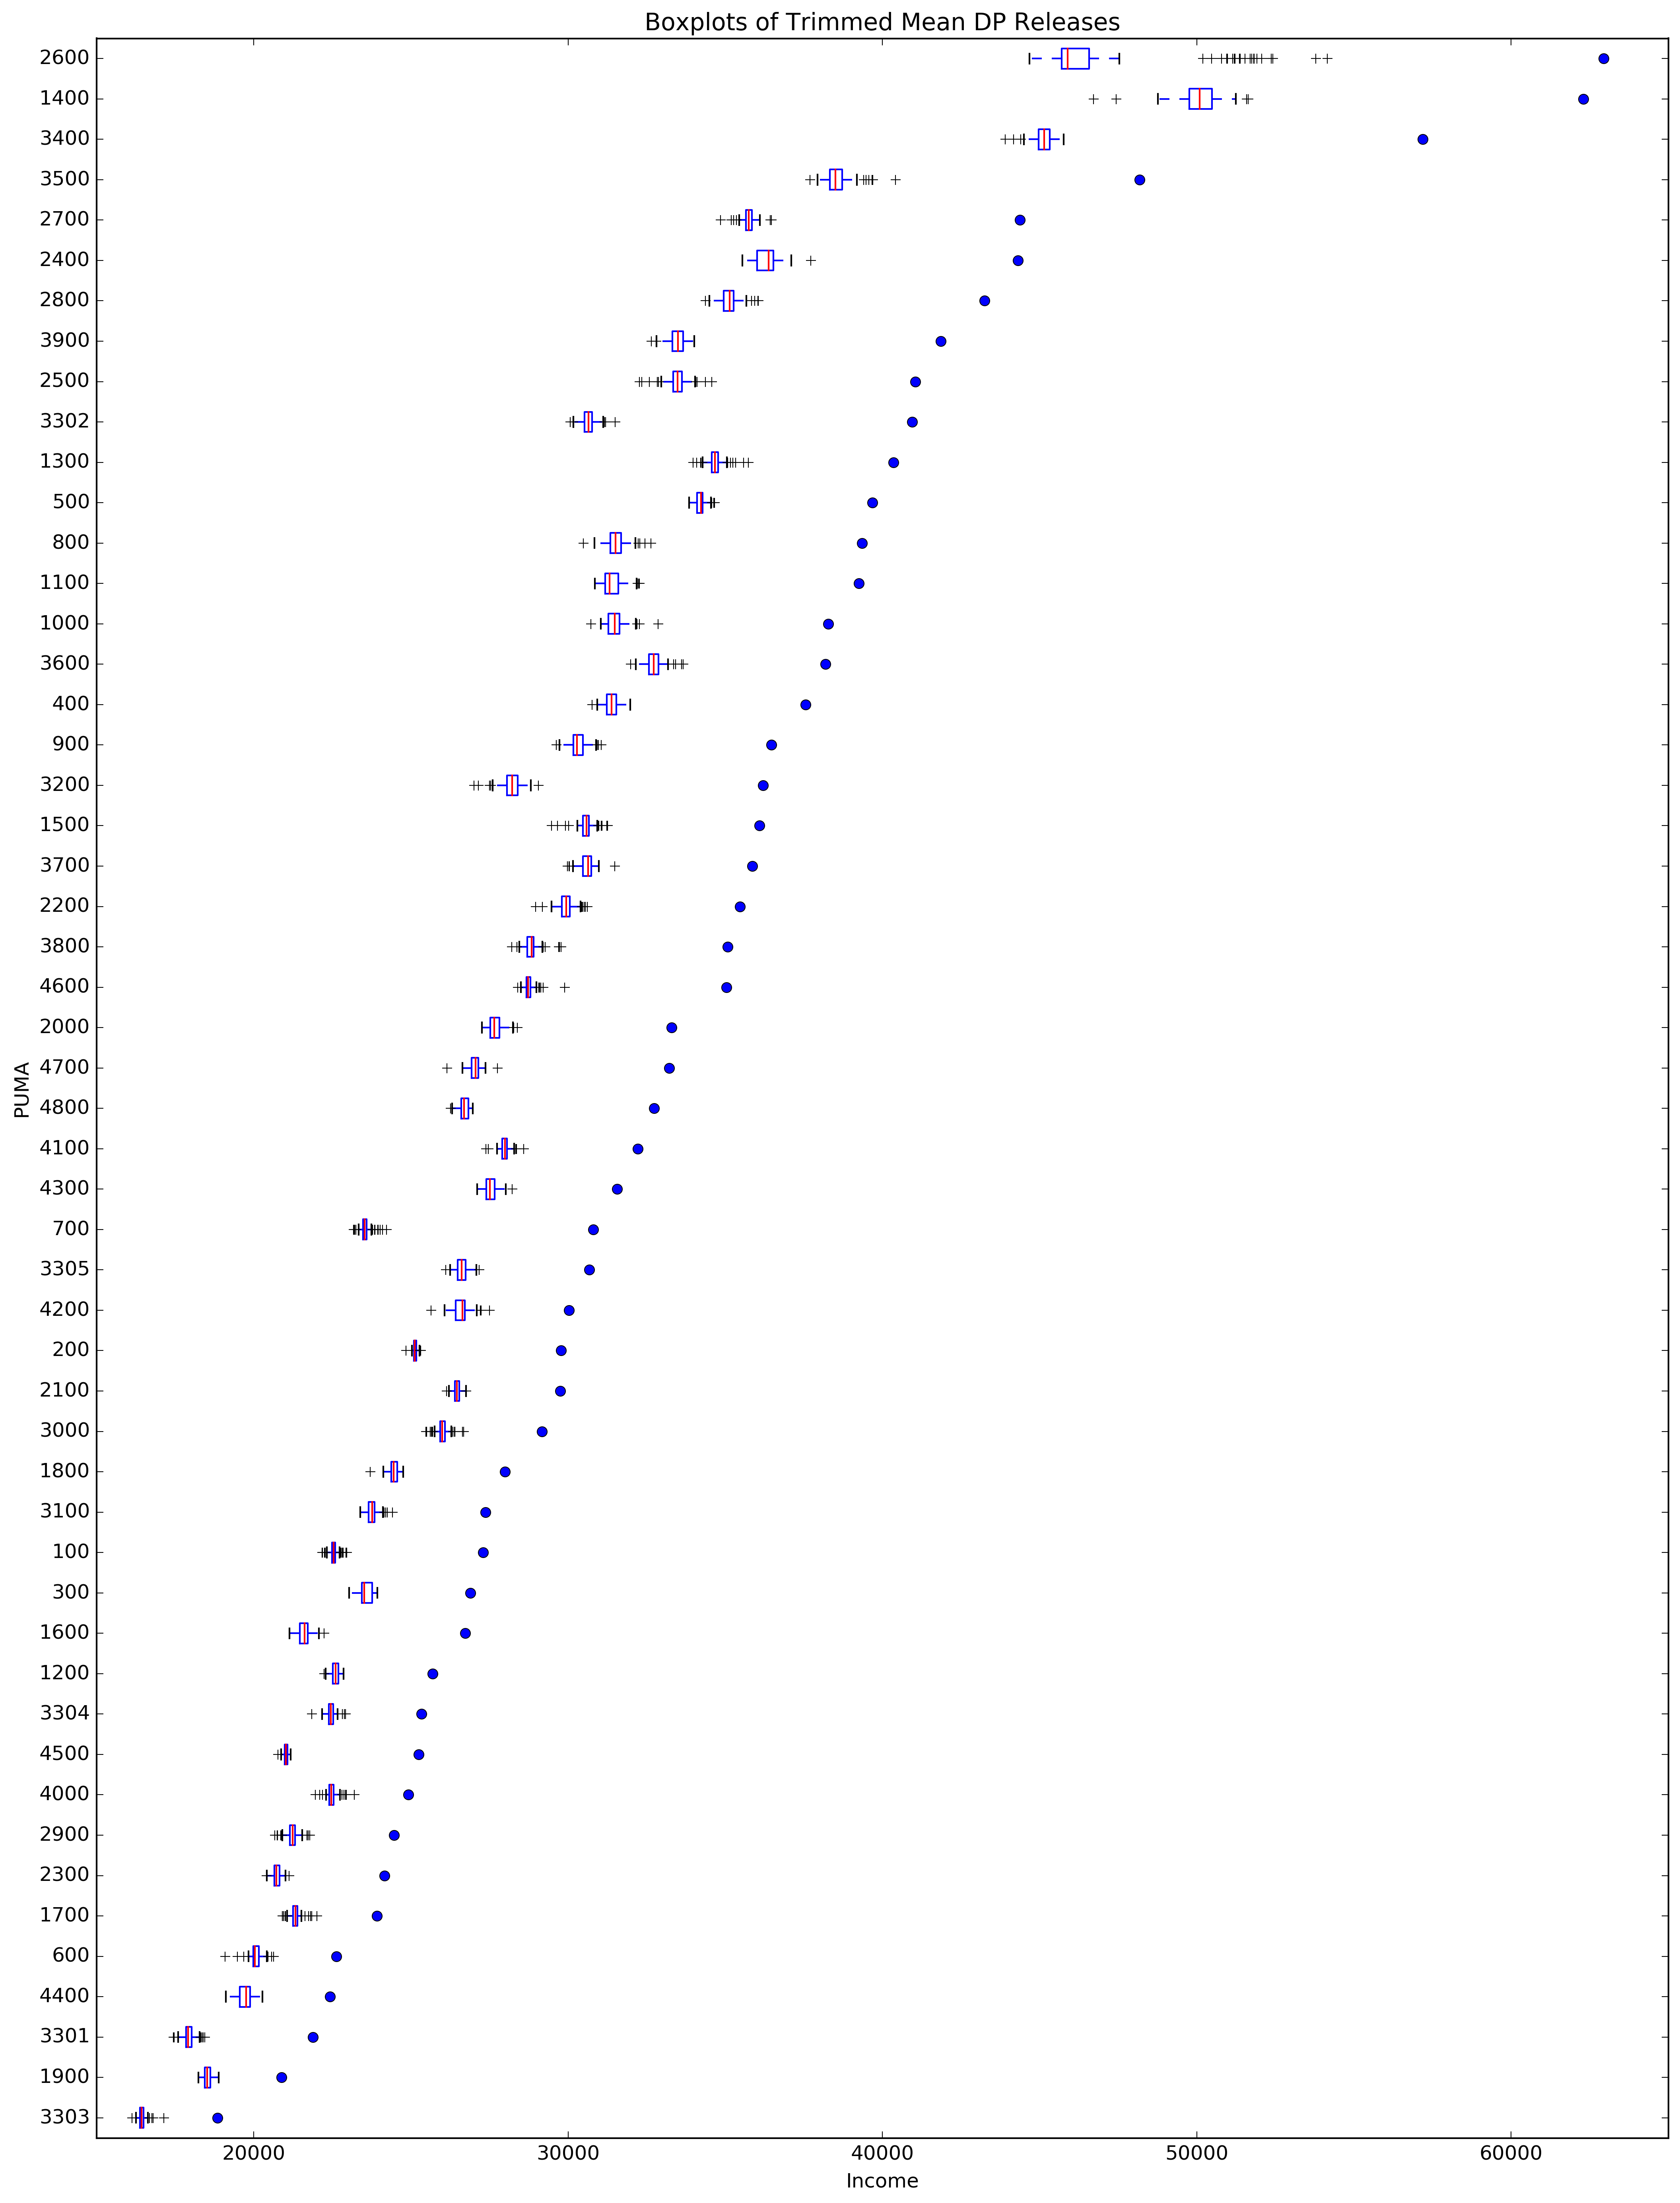
\includegraphics[scale=0.45]{trimmed_means_graph.png}

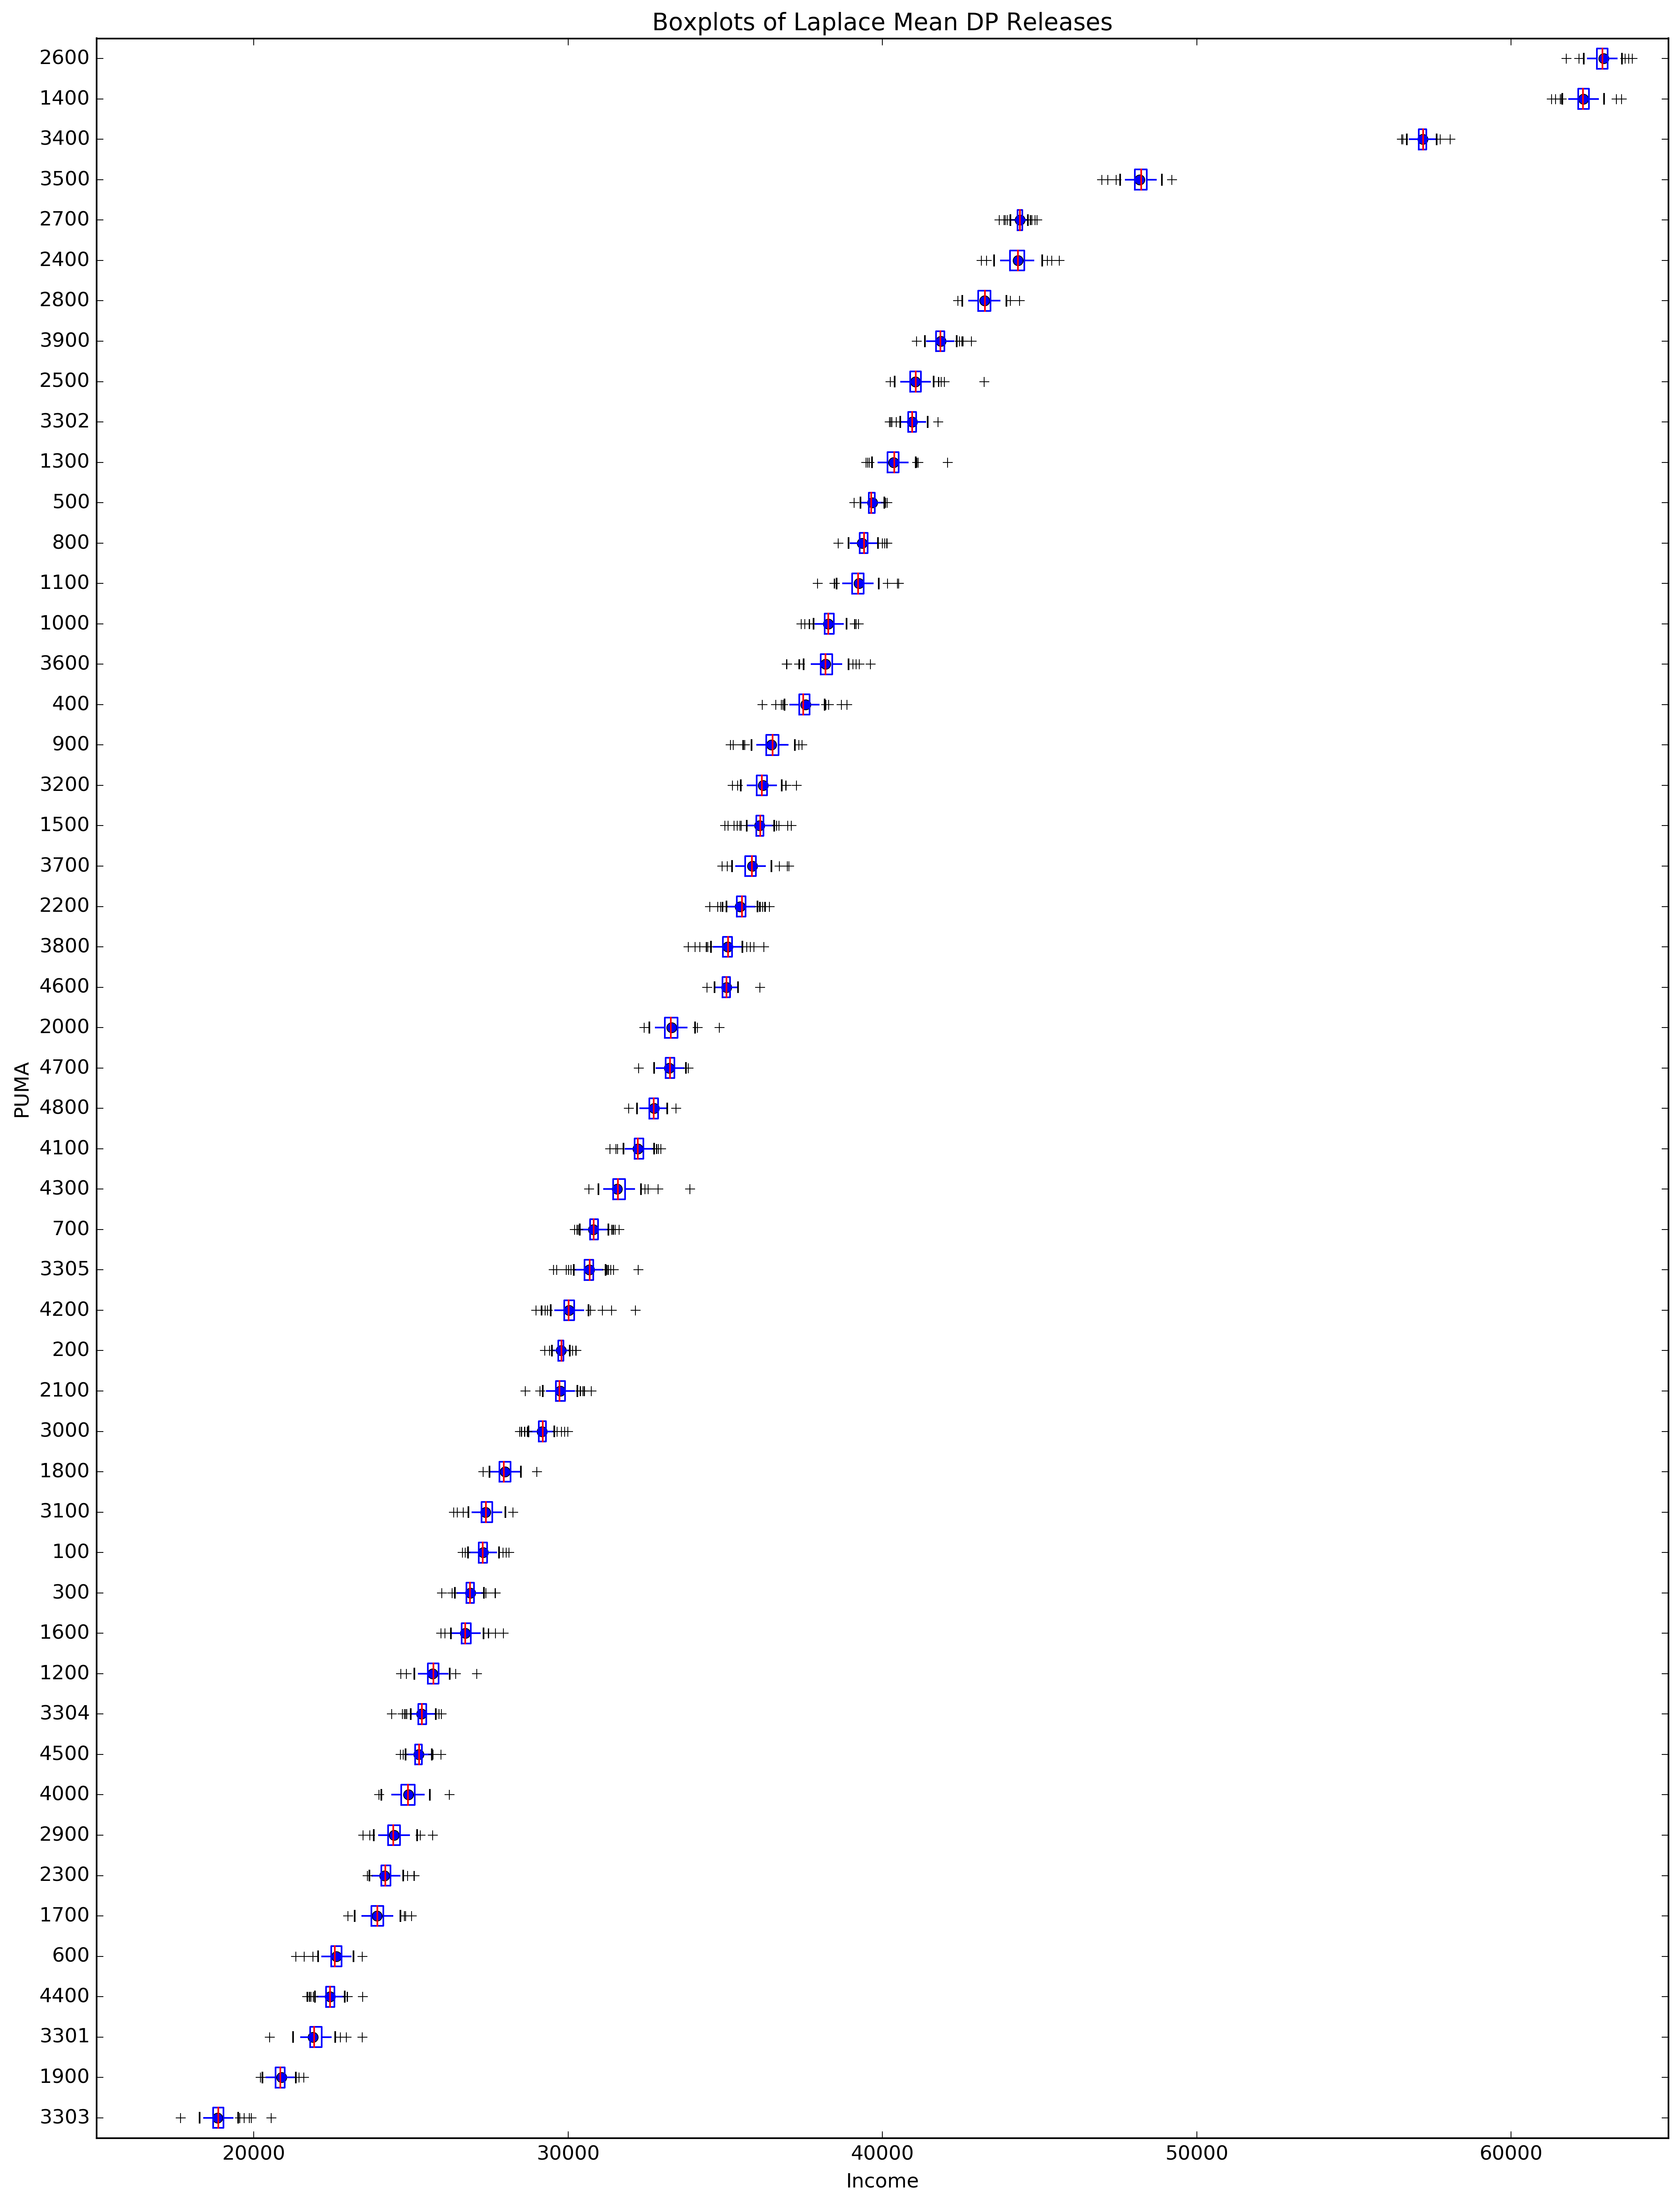
\includegraphics[scale=0.45]{laplace_means_graph.png}

\subsubsection{Analysis}

\noindent

Looking at our results, we see that the trimmed mean release, using our algorithm from Part 1d, consistently underestimates the true mean of the data. This makes sense because income data in America is highly skewed - there are a few high outliers that drive up the mean considerably. For example, according to \href{https://www2.census.gov/programs-surveys/cps/tables/time-series/historical-income-households/h05.xls}{2017 Census data}, the mean household income in the United States was \$86,220 while the median was \$61,372. Since our algorithm only calculates the mean for the households between our DP estimates of the 5th and 95th percent, it cuts out most of the high outliers, thus biasing the mean towards a lower value. We can see this effect in action when we look at the trend as mean income increases -- the greater the mean income, the more our algorithm tends to underestimate the mean. Additionally, as the mean income increases, our estimate of the 95th percentile varies more (presumably due to more variance in the numbers around the 95th percentile itself), and thus the variability of our releases increases greatly as well. This is quite noticeable in the difference of the size of the box plots for the PUMAs with the smallest means compared to those with the largest means.

\bigskip

As a result, the ordinary Laplace mechanism will perform better on skewed datasets, where one side has more outliers than the other. Our algorithm from 1d will perform better on symmetric datasets, especially those with high variance. By trimming out the outliers on each side, we can report a mean with less noise that is still accurate, as long as the dataset is symmetric. In order to increase the utility of our algorithm on skewed datasets such as these, we would need to adjust our dataset to be less skewed. Perhaps by performing some kind of transformation on the dataset that makes it more symmetrical, calculating our trimmed mean, then inverting the transformation, could we calculate a trimmed mean that is fairly accurate even on skewed data.

\newpage

\section{Problem 2}

\subsection{Process}

\noindent

Before plotting the results, we must calculate the different values of Laplace noise added under basic composition, the advanced composition theorem, and the ``optimal'' composition theorem used by PSI. Since I am more familiar with graphing in Python, I first wrote an R script to output the different $\epsilon$'s for different values of $k$ under PSI's optimal composition. This code is available in \cl{psi_epsilon.r}, located at Appendix \ref{appendix:psi_epsilon}.

\bigskip

Once I did this, I then generated the data for the basic and advanced composition theorems and graphed the results. This code is available in \cl{problem_2.py}, located at Appendix \ref{appendix:problem_2}.

\subsection{Plots}

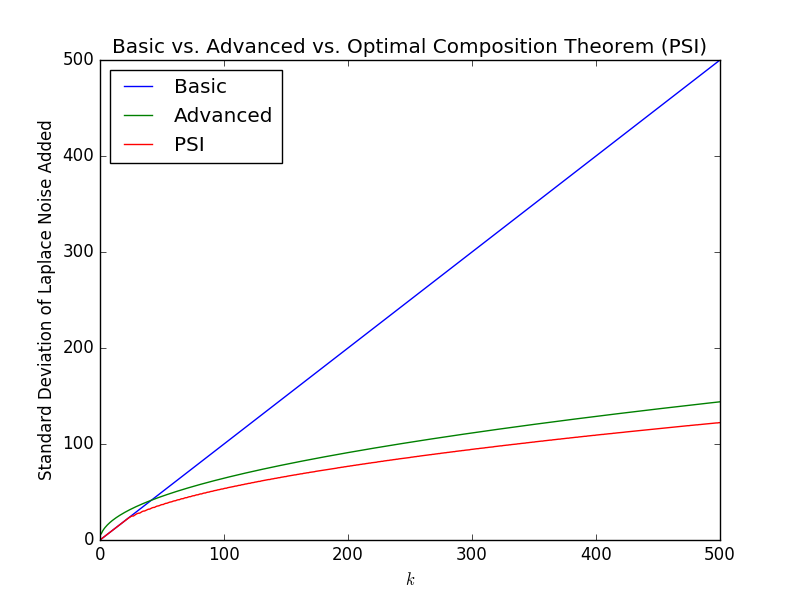
\includegraphics[scale=0.6]{problem_2_wide.png}

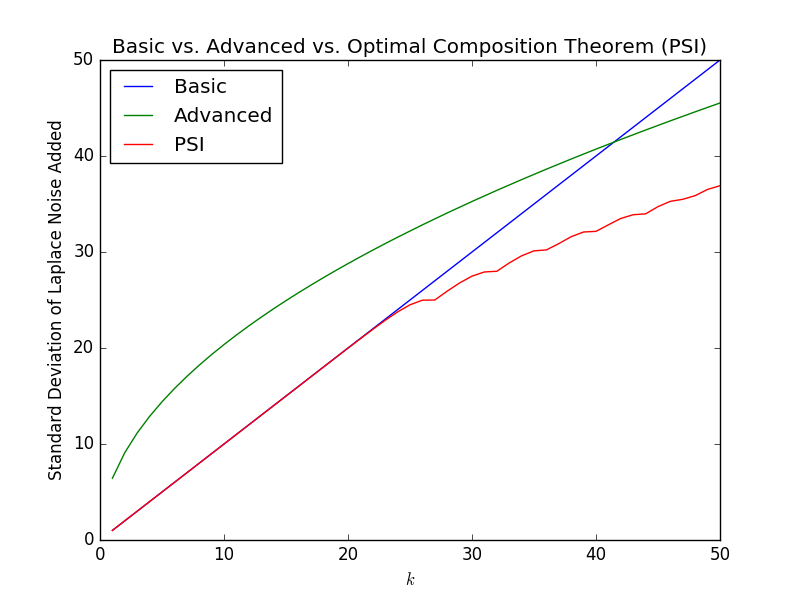
\includegraphics[scale=0.6]{problem_2_close.png}

\subsection{Results}

\noindent

Looking at the graphs, we can see how PSI's optimal composition always at least matches the other two composition theorems. It follows the basic composition theorem when it is optimal, then breaks away following a pattern similar to the advanced composition theorem when the advanced {}composition theorem becomes optimal. Looking at the results our script outputted, PSI strictly impoves upon the basic composition theorem when $k \geq 17$, while the advanced composition theorem strictly improves upon the basic composition theorem when $k \geq 42$.

\newpage

\section{Problem 3}

\subsection{Process}

\noindent

The code to calculate the bias and variance terms is available in \cl{problem_3.py}, located at Appendix \ref{appendix:problem_3}. The basic structure of the program is as follows:

\begin{itemize}
  \item For each of 100 trials:
  \begin{itemize}
    \item Generate a differentially private three-way histogram of income, education, and age
    \item Generate synthetic data based on that histogram
    \item Prune the real data to match the format of the synthetic data
    \item Bootstrap a dataset based on the real data, again to match the format of the synthetic data
    \item Calculate the beta coefficients for the synthetic, real, and bootstrapped data, and store them in a list
  \end{itemize}
  \item Calculate the bias squared and variance for both the synthetic and bootstrapped data
  \item Write the results out to a \cl{csv} file
\end{itemize}

\subsection{Results}

\noindent

Below is a table of the results for both the bootstrapped and synthetic data:

\begin{table}[h]
\begin{tabular}{|r|c|c|c|c|c|c|}
\hline
{\textbf{Type}} & $\beta_0$ Bias$^2$ & $\beta_0$ Variance & $\beta_1$ Bias$^2$ & $\beta_1$ Variance & $\beta_2$ Bias$^2$ & $\beta_2$ Variance \\ \hline
\textbf{Bootstrap} & 1.899E-07  & 1.042E-03 & 4.825E-12 & 4.576E-06 & 3.995E-10 & 1.186E-07 \\ \hline
\textbf{Synthetic} & 3.221E-02 & 8.888E-04 & 1.323E-04 & 4.004E-06 & 1.529E-06 & 1.038E-07 \\ \hline
\end{tabular}
\end{table}

\subsection{Analysis}

\noindent

Looking at the results, we see that the synthetic data has much higher bias than the bootstrapped data. This makes sense as we clipped our income fairly heavily by cutting out all negative numbers and clipping the top to $e^{12} \approx 162754$. This bias manifested itself in high (relative) bias terms for $\beta_0$, $\beta_1$, and $\beta_2$ compared to the respective terms for the bootstrapped dataset. It makes sense that the bias manifested itself relatively equally for each coefficient, because income was the only term that was clipped severly, while education and age weren't clipped at all (age was capped at 100, but such values are extremely rare). Additionally, we had to clip all negative counts to 0 when calculating probabilities to generate our synthetic dataset, which additionally biased this dataset.

\medskip

We also note that the variance for each synthetic coefficient is actually very slightly less than the variance for each respective bootstrapped coefficient. Reasoning about this, it makes sense that the variance of coefficients over such a large ($N = 241830$) generated dataset would not be any larger than that of a bootstrapped dataset. Since the noise added is symmetric, it should not affect the calculated regression coefficients much from iteration to iteration. As a result, the variance is virtually identical, and likely within the margin of error, of the variance of the bootstrapped coefficients.

\newpage

\begin{appendices}

\section{\cl{problem_1.py}}
\label{appendix:problem_1}

\begin{lstlisting}
"""
Andrew Shackelford
ashackelford@college.harvard.edu

CS 208 - Spring 2019
Homework 3, Problem 1
"""

import numpy as np
from scipy.special import softmax as softmax
import csv
import pickle
import matplotlib.pyplot as plt
import operator

# load and clean sample csv
def read_csv(file):
    with open(file, 'rU') as csv_file:
        reader = csv.DictReader(csv_file)
        data = []
        for row in reader:
            if row['englishability'] == 'NA':
                row['englishability'] = 2
            if row['income'][-4:] == 'e+05':
                row['income'] = int(row['income'][:-4]) * 100000
            for key in row.keys():
                row[key] = int(row[key])
            data.append(row)
        return data

# get the data split by a variable
def get_variable_data_by(data, variable, by):
    ret = {}
    for row in data:
        lst = ret.get(row[by], [])
        lst.append(row[variable])
        ret[row[by]] = lst
    return ret

# get the data split by a variable, clipped to a lower and upper bound
def get_variable_data_by_clip(data, variable, by, clip_l, clip_u):
    ret = get_variable_data_by(data, variable, by)
    for key in ret.keys():
        ret[key] = np.clip(ret[key], clip_l, clip_u)
    return ret

# calculate the sum of a dataset's points that are within certain bounds
def sum_within_bounds(x, lower, upper):
    sum_x = 0.
    for x_i in x:
        if x_i >= lower and x_i <= upper:
            sum_x += x_i
    return sum_x 

# utility function for any percentile
def utility(x, y, t):
    left_index = np.searchsorted(x, y, side='left')
    right_index = np.searchsorted(x, y, side='right')

    left_dist = np.abs(t * x.shape[0] - left_index)
    right_dist = np.abs(t * x.shape[0] - right_index)

    dist = min(left_dist, right_dist)
    # account for bias of left_index due to the way numpy insertion works
    if left_index <= t * x.shape[0]:
        dist += 1
    return x.shape[0] - dist

# mechanism for part a
def part_a(x, D, epsilon):
    p_05, p_95 = np.percentile(x, [5., 95.])

    # calculate mean for points within true percentiles
    n = float(len(x))
    sum_x = sum_within_bounds(x, p_05, p_95)
    mean_x = sum_x * (1. / (0.9 * n))

    # add sufficient noise
    scale = float(D) / (float(epsilon) * 0.9 * n)
    noise = np.random.laplace(scale=scale)

    return mean_x + noise

# mechanism for part c
def part_c(x, D, epsilon, t):
    global global_probabilities
    utilities = {}

    # create versions of x
    x_unique = np.unique(x)
    x_hash = hash(x.tostring())
    x_sorted = np.sort(x)

    # create variables for use in mechanism
    cur_x_idx = 0
    unique_count = x_unique.shape[0]
    unique_max = x_unique[-1]

    # only recalculate probabilities if needed
    if (x_hash, D, epsilon, t) not in global_probabilities:
        x = np.array(x)
        probabilities = []

        # use mechanism for sorted x that allows us to reduce number of weights calculated
        for d in range(D+1):
            if cur_x_idx >= unique_count:
                break
            if d >= x_unique[cur_x_idx]:
                utilities[d] = utility(x_sorted, d, t) * float(epsilon) / 2.
                cur_x_idx += 1

            probabilities.append(utilities[x_unique[cur_x_idx-1]])

        probabilities = softmax(probabilities)
        global_probabilities[(x_hash, D, epsilon, t)] = probabilities

    # calculate release
    p = global_probabilities[(x_hash, D, epsilon, t)]
    release = np.random.choice([d for d in range(unique_max+1)], p=p)
    return release

# mechanism for part d
def part_d(x, D, epsilon,):
    # calculate differentially private 5th and 95th percentiles
    local_ep = float(epsilon) / 3.
    p_05 = part_c(x, D, local_ep, 0.05)
    p_95 = part_c(x, D, local_ep, 0.95)

    # calculate sum within bounds for differentially private estimates
    n = float(len(x))
    sum_x = sum_within_bounds(x, p_05, p_95)
    mean_x = sum_x * (1. / (0.9 * n))

    # add noise
    scale = (3. * (p_95 - p_05)) / (0.9 * float(epsilon) * n)
    noise = np.random.laplace(scale=scale)

    return mean_x + noise

# calculate a differentially private mean using the standard Laplace mechanism
def standard_laplace_mean(x, D, epsilon):
    scale = float(epsilon) * float(D) / float(len(x))
    return np.mean(x) + np.random.laplace(scale=scale)

# function to perform the experiment for part f
def part_f_experiment():
    D = 1000000
    epsilon = 1.
    num_trials = 100

    # read in data, get both income and clipped income
    data = read_csv('MaPUMS5full.csv')
    income = get_variable_data_by(data, 'income', 'puma')
    clipped_income = get_variable_data_by_clip(data, 'income', 'puma', 0, D)

    true_means, trimmed_means, laplace_means = [], [], []
    true_mean = {}

    # calculate the true mean for each PUMA
    for key, array in income.iteritems():
        true_mean[key] = np.mean(array)
    true_means.append(true_mean)

    # for each trial
    for i in range(num_trials):
        trimmed_mean, laplace_mean = {}, {}

        # calculate the Trimmed and Laplace mean for each PUMA
        for key, array in clipped_income.iteritems():
            trimmed_mean[key] = part_d(array, D, epsilon)
            laplace_mean[key] = standard_laplace_mean(array, D, epsilon)

        trimmed_means.append(trimmed_mean)
        laplace_means.append(laplace_mean)

    # write the results out to file
    with open('true_means.pkl', 'wb') as f:
        pickle.dump(true_means, f)
    with open('trimmed_means.pkl', 'wb') as f:
        pickle.dump(trimmed_means, f)
    with open('laplace_means.pkl', 'wb') as f:
        pickle.dump(laplace_means, f)

def part_f_analysis():
    # read in the results
    with open('true_means.pkl', 'rb') as f:
        true_means = pickle.load(f)
    with open('trimmed_means.pkl', 'rb') as f:
        trimmed_means = pickle.load(f)
    with open('laplace_means.pkl', 'rb') as f:
        laplace_means = pickle.load(f)

    # create dictionaries for RMSE calculations
    trimmed_rmse = {puma:0. for puma in sorted(true_means[0].keys())}
    laplace_rmse = {puma:0. for puma in sorted(true_means[0].keys())}

    # sum the squared error for trimmed means
    for trimmed_mean in trimmed_means:
        for puma, mean in trimmed_mean.iteritems():
            trimmed_rmse[puma] += np.square(true_means[0][puma] - mean)

    # sum the squared error for Laplace means
    for laplace_mean in laplace_means:
        for puma, mean in laplace_mean.iteritems():
            laplace_rmse[puma] += np.square(true_means[0][puma] - mean)

    # take the mean and sqrt of trimmed SE
    for puma, rmse in trimmed_rmse.iteritems():
        trimmed_rmse[puma] = np.sqrt(rmse / float(len(trimmed_means)))

    # take the mean and sqrt of Laplace SE
    for puma, rmse in laplace_rmse.iteritems():
        laplace_rmse[puma] = np.sqrt(rmse / float(len(laplace_means)))

    # sort the PUMAs by their true means
    sorted_true_means = sorted(true_means[0].items(), key=operator.itemgetter(1))

    # print out LaTeX formatted results table
    print("\\hline")
    print("\\textbf{PUMA} & \\textbf{True Mean} \\textbf{Laplace RMSE} & \\textbf{Trimmed RMSE} \\\\ \\hline")
    for puma, _ in sorted_true_means:
        print(str(puma) + " & " +
              str(int(round(true_means[0][puma]))) + " & " +
              str(int(round(laplace_rmse[puma]))) + " & " +
              str(int(round(trimmed_rmse[puma]))) + " \\\\ \\hline")

# function to graph a boxplot
def graph(true_means, dp_means, puma_keys, title, file, xlim_l, xlim_u):
    fig, ax = plt.subplots(figsize=(17, 22))

    # create the boxplot data
    dp_boxplots = [[] for i in range(len(puma_keys))]
    for i in range(len(dp_means)):
        for j in range(len(puma_keys)):
            dp_boxplots[j].append(dp_means[i][puma_keys[j]])

    # draw the true mean data
    for j, puma in enumerate(puma_keys):
        ax.plot(true_means[0][puma], j+1, marker='o', color='blue')

    # draw the boxplot
    ax.boxplot(dp_boxplots, labels=puma_keys, vert=False)

    # add labels and save
    plt.ylabel('PUMA')
    plt.xlabel('Income')
    plt.title(title)
    plt.xlim(xlim_l, xlim_u)
    plt.savefig(file, bbox_inches='tight', dpi=300)

def part_f_graph():
    # load the data
    with open('true_means.pkl', 'rb') as f:
        true_means = pickle.load(f)
    with open('trimmed_means.pkl', 'rb') as f:
        trimmed_means = pickle.load(f)
    with open('laplace_means.pkl', 'rb') as f:
        laplace_means = pickle.load(f)

    # create variables
    sorted_true_means = sorted(true_means[0].items(), key=operator.itemgetter(1))
    puma_keys = [puma for puma, _ in sorted_true_means]

    # graph trimmed means
    graph(true_means=true_means,
          dp_means=trimmed_means,
          puma_keys=puma_keys,
          title="Boxplots of Trimmed Mean DP Releases",
          file="trimmed_means_graph.png",
          xlim_l=15000,
          xlim_u=65000)

    # graph Laplace means
    graph(true_means=true_means,
          dp_means=laplace_means,
          puma_keys=puma_keys,
          title="Boxplots of Laplace Mean DP Releases",
          file="laplace_means_graph.png",
          xlim_l=15000,
          xlim_u=65000)

def main():
    # create global probabilities dictionary
    global global_probabilities
    global_probabilities = {}

    # perform experiment, analysis, and graph
    part_f_experiment()
    part_f_analysis()
    part_f_graph()

if __name__ == "__main__":
    main()
\end{lstlisting}

\newpage

\section{\cl{psi_epsilon.r}}
\label{appendix:psi_epsilon}

{\lstset{frame=tb,
  language=R,
  aboveskip=3mm,
  belowskip=3mm,
  showstringspaces=false,
  columns=flexible,
  basicstyle={\small\ttfamily},
  numbers=none,
  numberstyle=\tiny\color{gray},
  keywordstyle=\color{blue},
  commentstyle=\color{dkgreen},
  stringstyle=\color{mauve},
  breaklines=true,
  breakatwhitespace=true,
  tabsize=3
}

\begin{lstlisting}
# Andrew Shackelford
# ashackelford@college.harvard.edu
#
# CS 208 - Spring 2019
# Homework 3, Problem 2

library("PSIlence")

epsilonGlobal <- 1
deltaGlobal <- 1e-9

# output dataframe
out <- rep(0, 500)

for (k in 1:500) {
  # for each k, calculate inverse matrix
  init <- rep(c(1/k, 0), k )
  params <- matrix(init, nrow=k, ncol=2, byrow=TRUE)
  inverse <- PSIlence:::update_parameters(params=params, hold=0, eps=epsilonGlobal, del=deltaGlobal)
  
  # since no parameters are held, each output row is the same, so just pick one
  out[k] <- inverse[1][1]
}

write.csv(out, file='psi_epsilon.csv')
\end{lstlisting}
}

\newpage

\section{\cl{problem_2.py}}
\label{appendix:problem_2}

\begin{lstlisting}
"""
Andrew Shackelford
ashackelford@college.harvard.edu

CS 208 - Spring 2019
Homework 3, Problem 2
"""

import csv
import numpy as np
import matplotlib.pyplot as plt

# read in the csv of psi epsilon_0 values
def read_csv(infile):
    with open(infile, 'rb') as f:
        next(f) # skip first line
        reader = csv.reader(f)
        x, y = [], []
        for row in reader:
            x.append(float(row[0]))
            y.append(float(row[1]))
    return x, y

# return the epsilon_0 under basic composition
def basic_composition(epsilon, k):
    return float(epsilon) / float(k)

# return the epsilon_0 under advanced composition
def advanced_composition(epsilon, delta, k):
    return float(epsilon) / np.sqrt(2 * float(k) * np.log(1./float(delta)))

# take an epsilon value and convert it to the appropriate laplace
# standard deviation for a count statistic, that is, invert it
def epsilon_to_std_dev(x):
    return 1. / float(x)

def main():
    # load and generate data
    psi_x, psi_y = read_csv('psi_epsilon.csv')
    basic_x, basic_y = [], []
    advanced_x, advanced_y = [], []
    for k in range(1, 501):
        basic_x.append(k)
        advanced_x.append(k)
        basic_y.append(basic_composition(1, k))
        advanced_y.append(advanced_composition(1, np.power(10., -9.), k))

    # convert epsilons to standard deviations
    basic_y = map(epsilon_to_std_dev, basic_y)
    advanced_y = map(epsilon_to_std_dev, advanced_y)
    psi_y = map(epsilon_to_std_dev, psi_y)

    # plot wide scale graph
    plt.plot(basic_x, basic_y, label='Basic')
    plt.plot(advanced_x, advanced_y, label='Advanced')
    plt.plot(psi_x, psi_y, label='PSI')
    plt.legend(loc='upper left')
    plt.title('Basic vs. Advanced vs. Optimal Composition Theorem (PSI)')
    plt.xlabel(r'$k$')
    plt.ylabel('Standard Deviation of Laplace Noise Added')
    plt.savefig('problem_2_wide.png')
    plt.clf()

    # plot close scale graph
    plt.plot(basic_x, basic_y, label='Basic')
    plt.plot(advanced_x, advanced_y, label='Advanced')
    plt.plot(psi_x, psi_y, label='PSI')
    plt.legend(loc='upper left')
    plt.title('Basic vs. Advanced vs. Optimal Composition Theorem (PSI)')
    plt.xlabel(r'$k$')
    plt.ylabel('Standard Deviation of Laplace Noise Added')
    plt.xlim((0, 50))
    plt.ylim((0, 50))
    plt.savefig('problem_2_close.png')

    # print out points where psi and advanced beat basic 
    advanced_found = False
    psi_found = False
    for k in range(1, 501):
        # account for floating point imprecision by using 0.0000001

        if basic_y[k-1] - advanced_y[k-1] > 0.0000001 and not advanced_found:
            print("advanced surpasses basic at k = " + str(k))
            advanced_found = True

        if basic_y[k-1] - psi_y[k-1] > 0.0000001 and not psi_found:
            print("psi surpasses basic at k = " + str(k))
            psi_found = True

if __name__ == "__main__":
    main()
\end{lstlisting}

\newpage

\section{\cl{problem_3.py}}
\label{appendix:problem_3}

\begin{lstlisting}
"""
Andrew Shackelford
ashackelford@college.harvard.edu

CS 208 - Spring 2019
Homework 3, Problem 3
"""

import numpy as np
import math
import csv

# load and clean sample csv
def read_csv(file, size=-1):
    with open(file, 'rU') as f:
        reader = csv.DictReader(f)
        data = []
        i = 0
        for row in reader:
            if i == size:
                break
            if row['englishability'] == 'NA':
                row['englishability'] = 2
            if row['income'][-4:] == 'e+05':
                row['income'] = int(row['income'][:-4]) * 100000
            for key in row.keys():
                row[key] = int(row[key])

            # change income to log(income)
            if row['income'] < 1:
                row['income'] = 1
            row['income'] = np.log(row['income'])

            data.append(row)
            i += 1
        return data

# write out histogram csv
def write_histogram_csv(results, file):
    with open(file, 'wb') as f:
        writer = csv.writer(f)
        writer.writerow(['income_bound_l', 'income_bound_r', 'educ_bound_l', 'educ_bound_r', 'age_bound_l', 'age_bound_r', 'value'])
        for row in results:
            writer.writerow(row)

# read in histogram csv
def read_histogram_csv(file):
    probabilities, bounds = [], []
    with open(file, 'rb') as f:
        reader = csv.DictReader(f)
        for row in reader:
            probabilities.append(float(row['value']))
            bound = [row['income_bound_l'], row['income_bound_r'], row['educ_bound_l'], row['educ_bound_r'], row['age_bound_l'], row['age_bound_r']]
            bounds.append(map(float, bound))
    return probabilities, bounds

# write out synthetic data csv
def write_data_csv(results, file):
    with open(file, 'wb') as f:
        writer = csv.writer(f)
        writer.writerow(['income', 'educ', 'age'])
        for row in results:
            writer.writerow(row)

# read in synthetic data csv as Xs and Ys
def read_data_csv(file):
    Xs, Ys = [], []
    with open(file, 'rb') as f:
        reader = csv.DictReader(f)
        for row in reader:
            Xs.append([1., float(row['educ']), float(row['age'])])
            Ys.append(float(row['income']))
    return Xs, Ys

# write out beta coefficient csv
def write_coefficient_csv(results, file):
    with open(file, 'wb') as f:
        writer = csv.writer(f)
        writer.writerow(['beta_0', 'beta_1', 'beta_2'])
        for row in results:
            writer.writerow(row)

# write out mse (bias and variance) csv
def write_mse_csv(results, file):
    with open(file, 'wb') as f:
        writer = csv.writer(f)
        writer.writerow(['type', 'bias_squared_0', 'bias_squared_1', 'bias_squared_2', 'variance_0', 'variance_1', 'variance_2'])
        for row in results:
            writer.writerow(row)

# clip a certain variable
def clip_data(data, variable, l, u):
    for row in data:
        if row[variable] < l:
            row[variable] = l
        if row[variable] > u:
            row[variable] = u

# get the bins for a given lower bound, upper bound, and number of bins
def get_bins(lower, upper, nbins):
    bins = np.linspace(lower, upper, num=nbins+1, dtype=int)
    bins = bins.astype(float)
    bins[-1] = bins[-1] + 0.0000001 # granularity
    return bins

# get the three-way histogram for a dataset
def get_histogram(data, income, educ, age, epsilon):
    # break down income, educ, and age into bounds and number of bins
    income_l, income_u, num_income_bins = income
    educ_l, educ_u, num_educ_bins = educ
    age_l, age_u, num_age_bins = age

    # generate the individual bins
    income_bins = get_bins(income_l, income_u, num_income_bins)
    educ_bins = get_bins(educ_l, educ_u, num_educ_bins)
    age_bins = get_bins(age_l, age_u, num_age_bins)

    # create the three-way bins
    bins = []
    for income_bin in income_bins:
        for educ_bin in educ_bins:
            for age_bin in age_bins:
                bins.append((income_bin, educ_bin, age_bin))
    num_bins = len(bins)

    # clip the data
    clip_data(data, 'income', income_l, income_u)
    clip_data(data, 'educ', educ_l, educ_u)
    clip_data(data, 'age', age_l, age_u)

    # calculate scale
    sensitivity = 2
    scale = sensitivity / epsilon

    true_dct = {}

    for row in data:
        # calculate which three-way bin a row should be in
        income_idx = int(np.floor((row['income']-income_l) * num_income_bins / (income_u - income_l)))
        educ_idx = row['educ'] - 1
        age_idx = int(np.floor((row['age']-age_l) * num_age_bins / (age_u - age_l)))

        # fix the granularity issues caused by upper bounds
        if row['income'] == income_u:
            income_idx = num_income_bins - 1
        if row['age'] == age_u:
            age_idx = num_age_bins - 1

        # calculate the bin bounds
        income_bound_l, income_bound_r = income_bins[income_idx], income_bins[income_idx+1]
        educ_bound_l, educ_bound_r = educ_bins[educ_idx], educ_bins[educ_idx+1]
        age_bound_l, age_bound_r = age_bins[age_idx], age_bins[age_idx+1]

        # enter the true results into the dictionary
        true_dct[(income_bound_l, income_bound_r, educ_bound_l, educ_bound_r, age_bound_l, age_bound_r)] = \
            true_dct.get((income_bound_l, income_bound_r, educ_bound_l, educ_bound_r, age_bound_l, age_bound_r), 0) + 1

    true_results, dp_results = [], []

    # calculate the true and DP results as rows
    for key, val in true_dct.iteritems():
        true_results.append((key[0], key[1], key[2], key[3], key[4], key[5], val))
        dp_results.append((key[0], key[1], key[2], key[3], key[4], key[5], val + np.random.laplace(scale=scale)))

    return dp_results, true_results

# Generate and write out the histograms
def generate_histograms():
    print("Generating histogram")
    data = read_csv('MaPUMS5full.csv')

    epsilon = 1.
    #format: lower, upper, num_bins
    income = 0, 12, 12 # lower bound of exp(0) = 1, upper bound of exp(12) = 162754
    educ = 1, 17, 16
    age = 0, 100, 20

    dp_results, true_results = get_histogram(data, income, educ, age, epsilon)

    write_histogram_csv(dp_results, 'dp_results.csv')
    write_histogram_csv(true_results, 'true_results.csv')

def generate_synthetic_data():
    print("Generating synthetic data")
    N = 241830

    # read in histogram results, clip the negative probabilities created by the DP noise, and normalize them
    probabilities, bounds = read_histogram_csv('dp_results.csv')
    probabilities = np.clip(probabilities, 0, None)
    probabilities = probabilities / np.linalg.norm(probabilities, ord=1)

    # generate the histogram indices to be used in the bootstrapped synthetic data
    indices = np.random.choice(len(bounds), N, replace=True, p=probabilities)

    synthetic_bounds = np.array(bounds)[indices, :]

    # generate the synthetic data
    synthetic_data = []
    for bounds in synthetic_bounds:
        income_bound_l, income_bound_r, educ_bound_l, educ_bound_r, age_bound_l, age_bound_r = bounds
        income = np.random.uniform(income_bound_l, income_bound_r)
        educ = educ_bound_l
        age = np.random.uniform(age_bound_l, age_bound_r)
        synthetic_data.append((income, educ, age))

    # write the results out to csv
    write_data_csv(synthetic_data, 'synthetic_data.csv')

# write out a csv of the true data in our desired format
def generate_true_data():
    print("Generating true data")
    data = read_csv('MaPUMS5full.csv')
    true_data = []
    for row in data:
        true_data.append((row['income'], row['educ'], row['age']))

    write_data_csv(true_data, 'true_data.csv')

# write out a csv of a bootstrap of the true data in our desired format
def generate_bootstrap_data():
    print("Generating bootstrap data")
    data = read_csv('MaPUMS5full.csv')
    indices = np.random.choice(len(data), len(data), replace=True)
    bootstrap_data = []
    for idx in indices:
        bootstrap_data.append((data[idx]['income'], data[idx]['educ'], data[idx]['age']))

    write_data_csv(bootstrap_data, 'bootstrap_data.csv')    

# calculate the linear regression coefficients for a given csv data file
def predict_coefficients(file):
    print ("Calculating coefficients for " + file)
    Xs, Ys = read_data_csv(file)
    Betas, residuals, ranks, s = np.linalg.lstsq(Xs, Ys)
    return Betas

# calculate the bias squared between two sets of betas
def calculate_bias_squared(betas_hat, betas):
    all_values = []
    for i in range(len(betas_hat)):
        all_values.append(betas_hat[i] - betas[i])
    return np.square(np.mean(all_values, axis=0))

# calculate the variance between two sets of betas
def calculate_variance(betas_hat, betas):
    all_values = []
    for i in range(len(betas_hat)):
        all_values.append(np.square(np.mean(betas_hat, axis=0) - betas_hat[i]))
    return np.mean(all_values, axis=0)

def main():
    num_trials = 100
    synthetic_betas, true_betas, bootstrap_betas = [], [], []

    # for each trial:
    # generate the histograms, data files, and predict coefficents
    for i in range(num_trials):
        print ("Running Trial " + str(i+1) + " of " + str(num_trials))

        generate_histograms()
        generate_synthetic_data()
        generate_true_data()
        generate_bootstrap_data()

        synthetic_betas.append(predict_coefficients('synthetic_data.csv'))
        true_betas.append(predict_coefficients('true_data.csv'))
        bootstrap_betas.append(predict_coefficients('bootstrap_data.csv'))

    # write out the coefficients to csvs
    write_coefficient_csv(synthetic_betas, 'synthetic_betas.csv')
    write_coefficient_csv(true_betas, 'true_betas.csv')
    write_coefficient_csv(bootstrap_betas, 'bootstrap_betas.csv')

    # calculate the bias squared and variance
    bootstrap_bias = calculate_bias_squared(bootstrap_betas, true_betas)
    bootstrap_variance = calculate_variance(bootstrap_betas, true_betas)
    synthetic_bias = calculate_bias_squared(synthetic_betas, true_betas)
    synthetic_variance = calculate_variance(synthetic_betas, true_betas)

    # write out the results to file
    results = [['bootstrap', bootstrap_bias[0], bootstrap_bias[1], bootstrap_bias[2], bootstrap_variance[0], bootstrap_variance[1], bootstrap_variance[2]],
               ['synthetic', synthetic_bias[0], synthetic_bias[1], synthetic_bias[2], synthetic_variance[0], synthetic_variance[1], synthetic_variance[2]]]
    write_mse_csv(results, 'problem_3_results.csv')

if __name__ == "__main__":
    main()
\end{lstlisting}

\end{appendices}

\end{document}